% SICACS / ICACS 2026 -- experimental (system + evaluation) paper in Springer LLNCS format
% Compile: pdflatex paper_experimental.tex  (run twice).  Figures are in figs_exp/.
% All numbers come from benchmark_out/, text_benchmark_out/ and benchmark_out/gradcam_attention.json.
%
\documentclass[runningheads]{llncs}
%
\usepackage[T1]{fontenc}
\usepackage{graphicx}
\usepackage{booktabs}
\usepackage{array}
\usepackage{url}
%
% ---- Grad-CAM attention numbers (filled from benchmark_out/gradcam_attention.json) ----
\newcommand{\gcRatioRes}{GC_RES_RATIO}
\newcommand{\gcRatioEff}{GC_EFF_RATIO}
\newcommand{\gcRealRes}{GC_RES_REAL}
\newcommand{\gcFakeRes}{GC_RES_FAKE}
\newcommand{\gcCorrRes}{GC_RES_CORR}
\newcommand{\gcWrongRes}{GC_RES_WRONG}
\newcommand{\gcN}{GC_N}
%
\begin{document}
%
\title{Evaluating Explainable Detectors for Deepfake Images, Fake News and Recruitment Scams: Cross-Dataset Generalisation and Attention Analysis}
%
\titlerunning{Explainable Detectors for Digital Deception}
%
\author{Harshida Joshi\inst{1}\orcidID{0009-0008-7301-4733} \and
Swati Sharma\inst{1} \and
Ashwini Kumar Jha\inst{1}\orcidID{0000-0002-6607-2168}}
%
\authorrunning{H. Joshi et al.}
%
\institute{Department of Artificial Intelligence \& Data Science,
Parul Institute of Engineering \& Technology,
Faculty of Engineering \& Technology,
Parul University, Waghodia, Vadodara, Gujarat, 391760, India\\
\email{harshidhijoshi@gmail.com, swati.sharma@paruluniversity.ac.in, ashwinibjha@gmail.com}}
%
\maketitle
%
\begin{abstract}
Deepfake images, fake news and fraudulent job advertisements are usually studied as separate classification problems, and detector accuracy is usually reported on the same corpus that was used for training. We implement one explainable pipeline for all three threats and evaluate each module under held-out and cross-dataset conditions. For synthetic face images, a fine-tuned ResNet50 reaches 89.9\% accuracy (AUC 0.967) on 6,000 held-out images and outperforms EfficientNetB0 (83.9\%), MobileNetV2 (82.7\%) and a CNN trained from scratch (59.0\%); an ablation shows that fine-tuning adds about three accuracy points. For fake news, TF-IDF classifiers reach 95.7--98.4\% on the corpus they were trained on, but fall to 82\% on a different news corpus and to chance level (45--48\%) on short fact-checked claims; the most influential terms are weekday names and reporting verbs, which indicates that the models learn journalistic style rather than veracity. For recruitment fraud, a linear model trained on EMSCAD attains F$_1$ = 0.80 on held-out postings, whereas a hand-written rule baseline attains 0.06. We replace heuristic explanations with Grad-CAM computed from the model gradients and with exact word contributions of the linear models, and we quantify attention: the ResNet50 places only a limited share of its Grad-CAM mass on the central face region. All experiments ran on a CPU-only machine with a 10\% training subsample, so we report them as a reproducible baseline rather than state-of-the-art results.
\keywords{DeepFake detection \and Fake news \and Recruitment fraud \and Grad-CAM \and Explainable AI \and Cross-dataset evaluation}
\end{abstract}
%
\section{Introduction}
A synthetic profile photograph, a rewritten news story and a fabricated job advertisement all exploit the same weakness: users cannot cheaply verify what they see. Research has progressed on each threat separately, with convolutional and transformer detectors for synthetic faces \cite{r02,r04,r10}, transformer and graph models for fake news \cite{r27,r32}, and a smaller literature on recruitment fraud \cite{r37,r38}. Two practical problems remain. First, accuracy is often reported on the corpus used for training, which hides how much a model has learned dataset-specific cues. Second, the explanations shown to users are frequently decorative rather than computed from the model, which makes them unreliable evidence \cite{r19}.

This paper evaluates a three-module pipeline with these problems in mind. Our contributions are:
\begin{enumerate}
\item A like-for-like comparison of four image classifiers (ResNet50, EfficientNetB0, MobileNetV2 and a small CNN) and an ablation of fine-tuning and augmentation on a 140,000-image real-versus-fake face dataset.
\item A cross-dataset study of fake-news classifiers on ISOT, WELFake and LIAR, with source tags that leak the label removed, showing a large generalisation gap.
\item A recruitment-scam classifier trained on EMSCAD, compared against the rule-based baseline from our earlier prototype.
\item Explanations that are computed from the models: Grad-CAM for the images (verified to reproduce the model output) and exact word contributions for the linear text models, together with a quantitative analysis of where the image model attends.
\end{enumerate}
We state the limits of the study plainly: training used a 10\% image subsample on a CPU, the text models are classical, and every number comes from a single training run.

\section{Related Work}
\textbf{Deepfake detection.} EfficientNet-family backbones with attention or frequency modules are common \cite{r02,r04}, ensembles and vision transformers are increasingly used \cite{r05,r10}, and surveys stress poor cross-generator generalisation \cite{r08,r09,r18}. Explainable detectors typically use Grad-CAM \cite{r07,r13,r39,gradcam}, but quantitative evaluation of explanations remains rare \cite{r19}.

\textbf{Fake news.} Work has moved from n-gram classifiers \cite{isot} to transformers, graph-augmented models and LLM-based augmentation \cite{r03,r27,r32,r36}; explanation methods such as LIME and SHAP are applied to BERT or LSTM models \cite{r26,r40,lime,shap}. Benchmarks differ widely in difficulty: fact-checked claims such as LIAR \cite{liar} are much harder than article-level corpora.

\textbf{Recruitment fraud.} Public data are scarce; EMSCAD \cite{emscad} is the standard corpus, and recent work applies tree ensembles and transformers \cite{r37,r38}. Few systems combine fraud detection with explanation.

\section{Datasets}
Table~\ref{tab:data} summarises the data. \emph{Faces:} 100,000 training, 20,000 validation and 20,000 test images, balanced between real and GAN-generated faces; real images come from Flickr-Faces-HQ \cite{ffhq}. \emph{ISOT} \cite{isot} contains 23,481 fake and 21,417 real articles; \emph{WELFake} \cite{welfake} merges four corpora (72,134 articles); \emph{LIAR} \cite{liar} has 12,836 PolitiFact statements with six truth labels, which we binarise (false, barely-true, pants-fire $\rightarrow$ fake). \emph{EMSCAD} \cite{emscad} contains 17,880 job postings of which 866 are fraudulent.

\textbf{Cleaning.} ISOT is known to be easy: 98.7\% of its real articles contain the string ``(Reuters)'' in the first 120 characters and none of the fake ones do. For ISOT and WELFake we therefore remove Reuters datelines, URLs and image-credit boilerplate, drop texts shorter than 15 words and remove exact duplicates (26\% of ISOT fake articles were duplicates). This leaves 38,794 ISOT and 63,092 WELFake articles. For EMSCAD, exact duplicates are removed (15,879 postings, 713 fraudulent) so that no posting appears in both training and test data. We split ISOT, WELFake and EMSCAD 70/15/15 with stratification; LIAR keeps its official split. WELFake's released labels are 1 = fake (37,106 rows) although its documentation states the opposite; we follow the row counts.

\begin{table}[t]
\caption{Data used. ``Used'' is the number actually used for training in the image task.}\label{tab:data}
\centering
\begin{tabular}{llrrr}
\toprule
Task & Dataset & Size & Train & Test \\
\midrule
Images & Real vs fake faces & 140,000 & 10,000 used (of 100,000) & 6,000 \\
Fake news & ISOT (cleaned) & 38,794 & 27,155 & 5,820 \\
Fake news & WELFake (cleaned) & 63,092 & 44,164 & 9,464 \\
Fake news & LIAR (binary) & 12,836 & 10,269 & 1,283 \\
Recruitment & EMSCAD (deduplicated) & 15,879 & 11,115 & 2,382 (107 scams) \\
\bottomrule
\end{tabular}
\end{table}

\section{Methods}
\subsection{Image classifiers}
All backbones are initialised from ImageNet weights \cite{resnet,effnet,mobilenet} except the small CNN (four conv blocks, 0.42M parameters), which is trained from scratch. A head of dropout (0.35), a 128-unit ReLU layer, dropout (0.25) and a sigmoid output gives the probability that an image is fake. Training has two stages: the backbone is frozen for four epochs (Adam, learning rate $10^{-3}$), then the last 40 backbone layers are unfrozen, with BatchNorm layers kept frozen, for two epochs at $10^{-5}$. We use early stopping and learning-rate reduction on validation loss, and mild augmentation (horizontal flip, rotation $\pm4\%$, zoom 8\%, contrast 10\%). Training uses 5,000 random real and 5,000 random fake images; validation and test use 3,000 random images per class from their own splits. Seeds are fixed.

\subsection{Text classifiers}
Fake news and recruitment texts are encoded with TF-IDF (word uni- and bigrams, sublinear term frequency, English stop words removed) and classified with L2-regularised logistic regression or a linear SVM, both with class weighting. For fake news we train on each corpus and test on all three. For recruitment, the decision threshold is tuned on the validation split only. The baseline is the rule set of our earlier prototype (payment, fee and urgency phrases); a posting is flagged when any rule fires. We also evaluate a random forest and report 5-fold cross-validated F$_1$ on the training portion.

\subsection{Explanations}
\textbf{Grad-CAM.} For the image models we compute the gradient of the fake probability with respect to the last convolutional feature map, average it spatially to obtain channel weights, and form the rectified weighted sum of channels \cite{gradcam}. Our implementation re-runs the saved model's preprocessing and head and we verified that it reproduces the model's own prediction to within $6\times10^{-7}$ for both ResNet50 and EfficientNetB0. \textbf{Word contributions.} For a linear model the decision score is the intercept plus the sum of weight$\times$TF-IDF value over terms, so each term's contribution is exact; this equals what SHAP's linear explainer reports up to a constant baseline \cite{shap}, and unlike LIME \cite{lime} it requires no sampling. \textbf{Attention measure.} Faces in the dataset are aligned crops, so the face lies near the centre. For \gcN{} test images per class we measure the fraction of Grad-CAM mass inside the central $50\%\times50\%$ window, which covers 25\% of the image; a value of 0.25 means uniform attention.

\subsection{Setup}
Experiments ran on a laptop with four CPU cores and 8~GB RAM, without a GPU, using TensorFlow 2.21 and scikit-learn 1.9. We report accuracy, precision, recall, F$_1$, ROC-AUC and, for the imbalanced recruitment task, PR-AUC. The positive class is ``fake'' or ``scam''. With 6,000 test images, the 95\% binomial confidence interval on an accuracy near 0.85 is about $\pm0.9$ points.

\section{Results}
\subsection{Deepfake image detection}
Table~\ref{tab:img} shows that ResNet50 is the strongest model (89.9\% accuracy, AUC 0.967), ahead of EfficientNetB0 and MobileNetV2, which are close to each other. The small CNN trained from scratch reaches only 59.0\%, which shows how much the pre-trained features contribute at this data size. The ablation (Table~\ref{tab:abl}) shows that fine-tuning adds about three points of accuracy. Augmentation did \emph{not} help: removing it raised accuracy from 83.9\% to 86.1\%. A plausible reason is the short schedule (six epochs on 10,000 images), in which augmentation slows convergence; we did not test longer schedules, so this should not be read as a general conclusion.

\begin{table}[t]
\caption{Image classifiers on 6,000 held-out test images (3,000 per class).}\label{tab:img}
\centering
\begin{tabular}{lrrrrrr}
\toprule
Model & Params & Acc. & Prec. & Rec. & F$_1$ & AUC \\
\midrule
ResNet50 & 23.9M & \textbf{0.899} & 0.925 & 0.868 & \textbf{0.896} & \textbf{0.967} \\
EfficientNetB0 & 4.2M & 0.839 & 0.854 & 0.817 & 0.835 & 0.923 \\
MobileNetV2 & 2.4M & 0.827 & 0.813 & 0.849 & 0.831 & 0.910 \\
Small CNN (scratch) & 0.4M & 0.590 & 0.572 & 0.716 & 0.636 & 0.633 \\
\bottomrule
\end{tabular}
\end{table}

\begin{table}[t]
\caption{Ablation on EfficientNetB0 (same test set).}\label{tab:abl}
\centering
\begin{tabular}{lrrr}
\toprule
Variant & Acc. & F$_1$ & AUC \\
\midrule
Full (fine-tuning + augmentation) & 0.839 & 0.835 & 0.923 \\
No fine-tuning & 0.809 & 0.805 & 0.894 \\
No augmentation & 0.861 & 0.863 & 0.938 \\
\bottomrule
\end{tabular}
\end{table}

\begin{figure}[t]
\centering
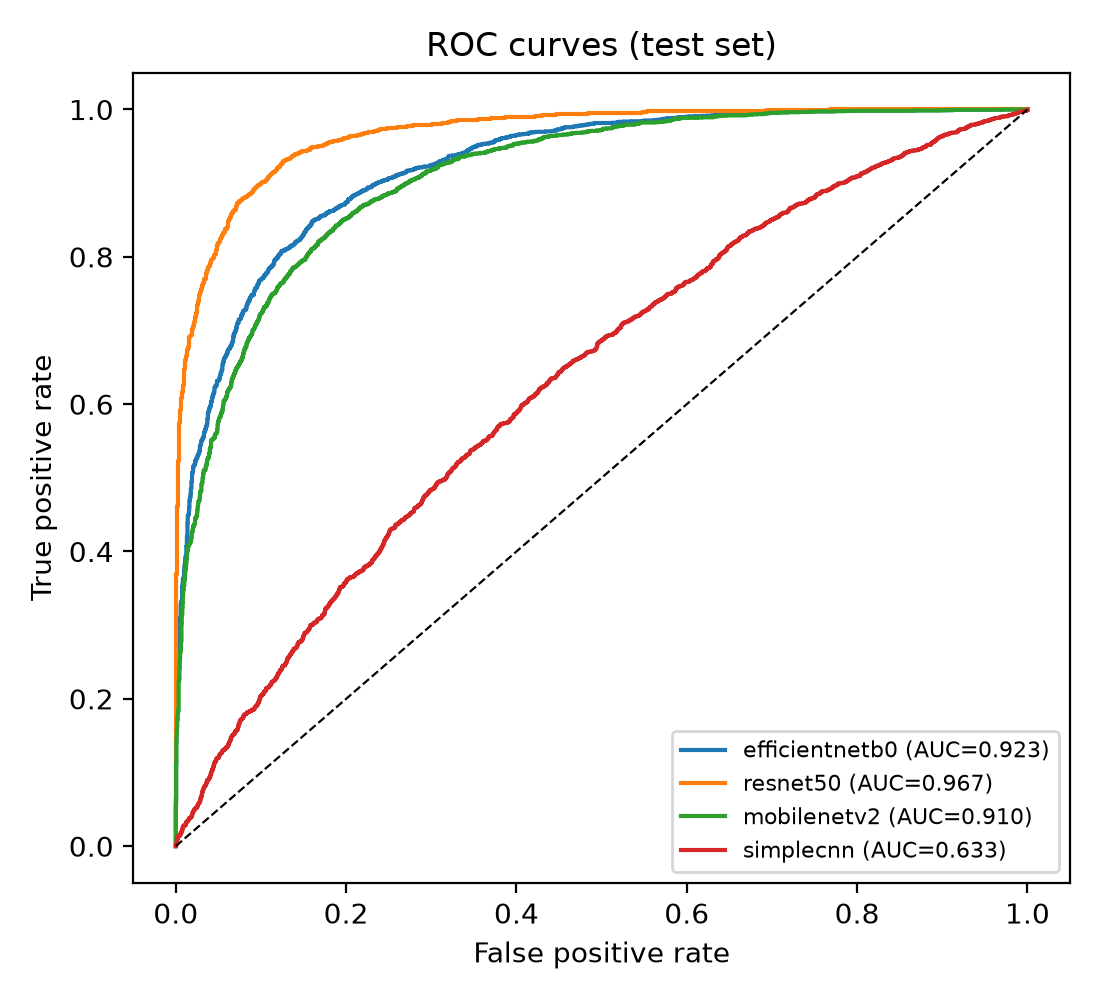
\includegraphics[width=0.62\textwidth]{figs_exp/roc_curves.png}
\caption{ROC curves of the image classifiers on the test set.}\label{fig:roc}
\end{figure}

\subsection{Fake news: in-domain accuracy does not transfer}
Table~\ref{tab:news} (logistic regression; the SVM is within 0.5 points) shows the central result. In-domain accuracy is high (98.4\% on ISOT, 95.7\% on WELFake) but drops to 82.2\% when the ISOT model is tested on WELFake, and both models are at or below chance on LIAR (44.7--48.4\%); a model trained on LIAR itself reaches 60.4\%, in line with the difficulty of that benchmark. The WELFake$\rightarrow$ISOT result (98.8\%) should not be read as generalisation, because WELFake merges sources of the same kind as ISOT and the corpora probably overlap.

The model weights explain the gap. The terms most associated with \emph{real} news are \texttt{said}, weekday names (\texttt{wednesday}, \texttt{tuesday}, \texttt{thursday}), \texttt{mr}, \texttt{percent} and \texttt{new york}; those most associated with \emph{fake} news are \texttt{video}, \texttt{watch}, \texttt{breaking}, \texttt{just} and \texttt{read}. These are cues of journalistic style and web formatting, not of truthfulness, and they are absent from one-sentence claims.

\begin{table}[t]
\caption{Fake-news logistic regression: accuracy / F$_1$ / AUC, rows = training set, columns = test set. Diagonal entries are in-domain.}\label{tab:news}
\centering
\begin{tabular}{lccc}
\toprule
Train $\backslash$ Test & ISOT & WELFake & LIAR \\
\midrule
ISOT & \textbf{.984} / .982 / .999 & .822 / .827 / .911 & .484 / .547 / .540 \\
WELFake & .988 / .986 / .999 & \textbf{.957} / .952 / .992 & .447 / .582 / .526 \\
LIAR & .592 / .586 / .637 & .581 / .566 / .619 & \textbf{.604} / .549 / .642 \\
\bottomrule
\end{tabular}
\end{table}

\subsection{Recruitment-scam detection}
Table~\ref{tab:job} shows that the rule baseline is at chance (ROC-AUC 0.506, F$_1$ 0.06): its payment and fee patterns, written for a different style of scam, almost never match EMSCAD's English postings. The trained linear models reach F$_1$ of 0.80--0.81 (5-fold cross-validated F$_1$ 0.83--0.85), and the random forest is weaker (0.73). Dropping the structured fields (logo, questions, salary) leaves F$_1$ unchanged at 0.80, so the text-only model, which is the one a web form can supply, is deployed. The test set contains only 107 fraudulent postings, so recall (0.72) carries a wide uncertainty (roughly $\pm0.08$). Terms pointing toward scam include \texttt{data entry}, \texttt{earn}, \texttt{money} and \texttt{clerical}; several others are company-specific (for example \texttt{accion}), which suggests the model partly memorises employers in this corpus.

\begin{table}[t]
\caption{Recruitment-scam detection on EMSCAD (2,382 test postings, 107 scams; scam = positive).}\label{tab:job}
\centering
\begin{tabular}{lrrrrr}
\toprule
Model & Prec. & Rec. & F$_1$ & PR-AUC & ROC-AUC \\
\midrule
Rule-based baseline & 0.056 & 0.065 & 0.060 & 0.046 & 0.506 \\
TF-IDF + logistic regression & 0.868 & 0.738 & 0.798 & 0.866 & 0.987 \\
TF-IDF + linear SVM & 0.907 & 0.729 & \textbf{0.808} & \textbf{0.875} & 0.987 \\
Random forest & 0.779 & 0.692 & 0.733 & 0.816 & 0.975 \\
Logistic regression, text only (deployed) & 0.895 & 0.720 & 0.798 & 0.837 & 0.963 \\
\bottomrule
\end{tabular}
\end{table}

\subsection{Where does the image model look?}
GC_ATTENTION_PARAGRAPH

\subsection{Implementation}
The detectors are served by a Django web application. The earlier prototype labelled an edge-based saliency map as Grad-CAM and word-frequency heuristics as LIME and SHAP; both were replaced by the computed explanations described above, and inputs shorter than 30 words receive a reliability warning because the fake-news model is near chance on short claims.

\section{Discussion and Limitations}
\textbf{Reduced data and compute.} The image models saw 10\% of the training images, and all runs are CPU-only, so absolute accuracies are probably below what the same methods reach on a GPU with all 100,000 images; the ranking of models and the ablation conclusions may also change. \textbf{Single runs.} Each configuration was trained once; differences of one or two points, such as the augmentation result, are within what seed variation could produce. \textbf{Classical text models.} The text modules use TF-IDF with linear models; we did not train transformer models, which are the usual choice in recent work \cite{r27,r38}, so we make no claim about their cross-dataset behaviour. \textbf{Dataset effects.} The face images are aligned crops from one data source, so the image results do not establish robustness to other generators, compression or in-the-wild photographs. EMSCAD has few positives and company-specific cues. Our generalisation findings for fake news are consistent with the view that article-level style, not veracity, drives high in-domain scores.

\section{Conclusion}
A single explainable pipeline for deepfake images, fake news and recruitment scams is feasible on modest hardware, but evaluation protocol matters more than model choice. ResNet50 gave the best image results; fake-news accuracy collapsed across corpora and on claim-level data; and a learned recruitment model clearly beat hand-written rules. Replacing decorative explanations with computed ones exposed how the models actually behave. Future work will train on the full image set with a GPU, add transformer baselines for text, test other generators and measure explanation faithfulness with deletion and insertion tests.

\begin{thebibliography}{99}
\bibitem{r02}
M. Kumar, A. Kumar, V. Yadav, et al: A hybrid spatial–frequency attention-based algorithm using efficientnet for robust and interpretable deepfake detection. Scientific Reports, 16(1) (2026). \doi{10.1038/s41598-026-46086-9}

\bibitem{r04}
B. G. Deepa, C. K. Lokesh, D. Umamaheswari, et al: An enhanced deep learning framework for DeepFake detection using EfficientNet-B3 comparative evaluation of deep and machine learning techniques. Discover Computing, 29(1) (2026). \doi{10.1007/s10791-025-09890-x}

\bibitem{r10}
A. H. Soudy, O. Sayed, H. Tag-Elser, et al: Deepfake detection using convolutional vision transformers and convolutional neural networks. Neural Computing and Applications, 36(31), 19759–19775 (2024). \doi{10.1007/s00521-024-10181-7}

\bibitem{r27}
H. Rama Moorthy, N. J. Avinash, N. S. Krishnaraj Rao, et al: Dual stream graph augmented transformer model integrating BERT and GNNs for context aware fake news detection. Scientific Reports, 15(1) (2025). \doi{10.1038/s41598-025-05586-w}

\bibitem{r32}
C. Kumar, M. Bansal, M. A. Khan, et al: Graph-augmented transformer ensemble framework for robust and scalable fake news detection in social media ecosystems. Scientific Reports, 16(1) (2025). \doi{10.1038/s41598-025-31653-3}

\bibitem{r37}
M. Naudé, K. J. Adebayo, R. Nanda: A machine learning approach to detecting fraudulent job types. AI & SOCIETY, 38(2), 1013–1024 (2023). \doi{10.1007/s00146-022-01469-0}

\bibitem{r38}
K. Taneja, J. Vashishtha, S. Ratnoo: Fraud-BERT: transformer based context aware online recruitment fraud detection. Discover Computing, 28(1) (2025). \doi{10.1007/s10791-025-09502-8}

\bibitem{r19}
K. Tsigos, E. Apostolidis, S. Baxevanakis, et al: Towards Quantitative Evaluation of Explainable AI Methods for Deepfake Detection. 3rd ACM International Workshop on Multimedia AI against Disinformation, 37–45 (2024). \doi{10.1145/3643491.3660292}

\bibitem{r05}
K. Omar, R. H. Sakr, M. F. Alrahmawy: An ensemble of CNNs with self-attention mechanism for DeepFake video detection. Neural Computing and Applications, 36(6), 2749–2765 (2024). \doi{10.1007/s00521-023-09196-3}

\bibitem{r08}
B. C. Soundarya, H. L. Gururaj: Deepfake detection: critical review of state-of-the-art approaches and future perspectives. Discover Applied Sciences, 8(2) (2026). \doi{10.1007/s42452-025-08174-9}

\bibitem{r09}
N. A. Bhat, K. J. Giri: DeepFake detection in images and videos: a survey on models, datasets, and evaluation metrics. Multimedia Tools and Applications, 85(3) (2026). \doi{10.1007/s11042-026-21365-9}

\bibitem{r18}
Y. Mirsky, W. Lee: The Creation and Detection of Deepfakes. ACM Computing Surveys, 54(1), 1–41 (2022). \doi{10.1145/3425780}

\bibitem{r07}
F. Castro, V. Gattulli, D. Impedovo, et al: DeepDect: an explainable AI platform for face swapping and face generation DeepFake detection. Multimedia Tools and Applications, 85(5) (2026). \doi{10.1007/s11042-026-21672-1}

\bibitem{r13}
N. Mansoor, A. I. Iliev: Explainable AI for DeepFake Detection. Applied Sciences, 15(2), 725 (2025). \doi{10.3390/app15020725}

\bibitem{r39}
DeepFake Detection Using CNN Models with Explainable AI Techniques: IEEE Access (2025). \doi{10.1109/ACCESS.2025.11135663}

\bibitem{gradcam}
R. R. Selvaraju, M. Cogswell, A. Das, R. Vedantam, D. Parikh, D. Batra: Grad-CAM: visual explanations from deep networks via gradient-based localization. In: Proc. IEEE International Conference on Computer Vision (ICCV), pp. 618--626 (2017).

\bibitem{isot}
H. Ahmed, I. Traore, S. Saad: Detection of online fake news using N-gram analysis and machine learning techniques. In: Intelligent, Secure, and Dependable Systems in Distributed and Cloud Environments (ISDDC 2017), LNCS 10618, pp. 127--138. Springer (2017).

\bibitem{r03}
R. Chalehchaleh, R. Farahbakhsh, N. Crespi: Addressing data scarcity in multilingual fake news detection: an LLM-based dataset augmentation approach. Social Network Analysis and Mining, 15(1) (2025). \doi{10.1007/s13278-025-01505-z}

\bibitem{r36}
B. S. Alqadi, S. A. Alsuhibany, S. N. Yousafzai, et al: Transfer learning driven fake news detection and classification using large language models. Scientific Reports, 15(1) (2025). \doi{10.1038/s41598-025-10670-2}

\bibitem{r26}
S. G. Sneha, A. Sen, S. Malik, et al: BiLSTM-LIME: integrating NLP and advanced machine learning models for fake news detection. Discover Artificial Intelligence, 6(1) (2026). \doi{10.1007/s44163-026-00852-w}

\bibitem{r40}
X. Men, V. Y. Mariano: Explainable Fake News Detection Based on BERT and SHAP Applied to COVID-19. International Journal of Modern Education and Computer Science, 16(1), 11–22 (2024). \doi{10.5815/ijmecs.2024.01.02}

\bibitem{lime}
M. T. Ribeiro, S. Singh, C. Guestrin: ``Why should I trust you?'' Explaining the predictions of any classifier. In: Proc. 22nd ACM SIGKDD International Conference on Knowledge Discovery and Data Mining, pp. 1135--1144 (2016).

\bibitem{shap}
S. M. Lundberg, S.-I. Lee: A unified approach to interpreting model predictions. In: Advances in Neural Information Processing Systems 30 (NeurIPS), pp. 4765--4774 (2017).

\bibitem{liar}
W. Y. Wang: ``Liar, liar pants on fire'': a new benchmark dataset for fake news detection. In: Proc. 55th Annual Meeting of the Association for Computational Linguistics (Short Papers), pp. 422--426 (2017).

\bibitem{emscad}
S. Vidros, C. Kolias, G. Kambourakis, L. Akoglu: Automatic detection of online recruitment frauds: characteristics, methods, and a public dataset. Future Internet, 9(1), 6 (2017).

\bibitem{ffhq}
T. Karras, S. Laine, T. Aila: A style-based generator architecture for generative adversarial networks. In: Proc. IEEE/CVF Conf. Computer Vision and Pattern Recognition (CVPR), pp. 4401--4410 (2019).

\bibitem{welfake}
P. K. Verma, P. Agrawal, I. Amorim, R. Prodan: WELFake: word embedding over linguistic features for fake news detection. IEEE Transactions on Computational Social Systems, 8(4), 881--893 (2021).

\bibitem{resnet}
K. He, X. Zhang, S. Ren, J. Sun: Deep residual learning for image recognition. In: Proc. IEEE Conf. Computer Vision and Pattern Recognition (CVPR), pp. 770--778 (2016).

\bibitem{effnet}
M. Tan, Q. V. Le: EfficientNet: rethinking model scaling for convolutional neural networks. In: Proc. 36th International Conference on Machine Learning (ICML), PMLR 97, pp. 6105--6114 (2019).

\bibitem{mobilenet}
M. Sandler, A. Howard, M. Zhu, A. Zhmoginov, L.-C. Chen: MobileNetV2: inverted residuals and linear bottlenecks. In: Proc. IEEE Conf. Computer Vision and Pattern Recognition (CVPR), pp. 4510--4520 (2018).

\end{thebibliography}
\end{document}
